This section shows an application of the scaled logit model to the Ha Nam cohort which is plotted in Figure \ref{HanamCounts}. For this cohort, the Cox model is not suitable due to absence of reliable data on disease activity. The standard logistic model is inappropriate due to unjustified assumption of baseline of 1.

\begin{figure}[htp]
	\centering
	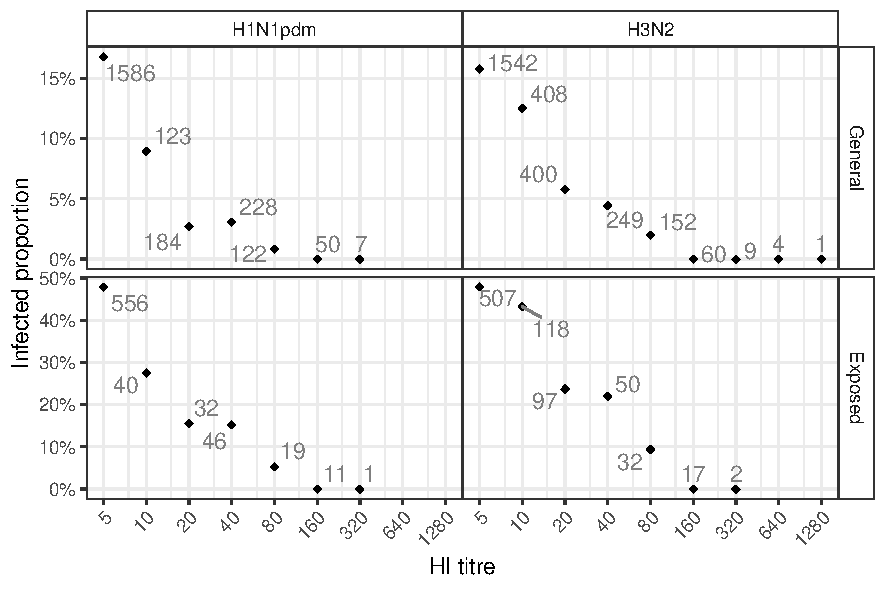
\includegraphics[width=0.9\textwidth]{../data-plot/hanam-hi-summ-light.pdf}
	\caption{
	Ha Nam cohort data. Subjects were grouped by virus and measured HI titre. Numbers next to points are the total number of observations in the corresponding group. The top row is all observations. The bottom row are the observations from households with at least one infection in a given season. The left column is observations for the H1N1pdm virus, the right row --- for H3N2 virus.
	}
	\label{HanamCounts}
\end{figure}
